\documentclass{ximera}

\graphicspath{     %% setup a global graphics path
{./}               %% look in the same-level directory
{./pictures/}      %% look in graphics
{../pictures/}     %% look up one directory, then in graphics
%{../../pictures/} %% look up two directories, then in graphics
}

\author{Zack Reed}
%%Snapp, B. (2024). Ximera la-carte: An open-source platform for interactive textbooks. https://ximera.osu.edu
%%OpenAI. (2023). ChatGPT (Mar 14 version) [Large language model]. https://chat.openai.com/chat

\title{Learning Activity: Vectors are Everywhere!}

\begin{document}
\begin{abstract}
    An introduction to how vectors provide a lens for understanding the world around us.
\end{abstract}
\maketitle


\section{Vectors and the World Around Us}

While the ``are" in the phrase ``Vectors are Everywhere" is slightly hyperbolous, it's not far from the truth. 

More accurately, we ``can" use vectors to represent just about anything in the world around us, as long as we're smart about it. Here we'll begin a book-long exploration of the ways that we've found it useful to represent the world around us through vectors. 

You'll see lots of vagueries that we'll make more precise as we go along!

\begin{remark}\name{Initial Terminology}

  To start, we'll give brief definitions of vectors and scalars, but then save more formal mathematical analyses until later. First, we'll focus on the utility of vectors in representing the world around us.

  The main three ways to initially think about vectors are as: 1) arrays of numbers, 2) arrows in space, and 3) quantities that you can add and scalar multiply.

  \begin{definition}{Scalars}

    For now, we're going to think of \textbf{scalars} as real numbers. $1$, $100$, $\pi$, $e^2$, are all examples of scalars.

  \end{definition}

  \begin{definition}{Vectors as Addition and Scalar Multiplication}

    Vectors, thought of most abstractly, are quantities where addition and scalar multiplication make sense. We'll get more precise about this later, but for now we're going to call a collection of vectors a \textit{vector space} if for $\vec{v}$ and $\vec{w}$ in the space, $a\vec{v}+b\vec{w}$ is also in the space for all scalars $a$ and $b$. We would call $\vec{v}$ and $\vec{w}$ \textit{vectors}.

  \end{definition}

\end{remark}


\begin{exploration}\name{Thinking About Data: An Apple a Day}

Consider the apple in the image below. What about this apple can we represent numerically?

\begin{center}
  \includegraphics[width=.5\textwidth]{apple-1.jpeg}
  %Generated by "Playground" AI, playground.com/create
\end{center}

\begin{selectAll}
    \choice[correct]{The apple's weight}
    \choice[correct]{The apple's color}
    \choice[correct]{The apple's volume}
    \choice{The apple's taste}
    \choice[correct]{The length of the apple's stem}
    \choice[correct]{The circumference of the largest horizontal cross-section of the apple}
    \choice{How the apple smells}
\end{selectAll}
\end{exploration}

In order to figure out how we can use vectors to say meaningful things about fruit, like this apple, we first need to get some common terminology and visualization down.

\begin{remark}

  Let's start with some basic terminology. 

\begin{definition}
    \item[Tuples] We can organize the measurements of the apple by encoding values of the apple's useful features as the locations in space. This is what's called a tuple, or more specifically an \textit{ordered tuple}. We more colloquially call these \textit{points} in space, however depending on the context you can equally call them \textit{vectors}.


    \item[An ordered pair] is just a pair of numbers $[a,b]$ delineated by parenthesis (or brackets) with the entries separated by a comma. It's called ``ordered'' because $[a,b] \ne [b,a]$. 
    
    \begin{example}

      In terms of vectors, if $\vec{v}=[3,4]$ and $\vec{w}=[4,3]$, then $\vec{v}\ne \vec{w}$, because the first coordinate of $\vec{v}$ is $3$ and the first coordinate of $\vec{w}$ is $4$.

    \end{example}
    
    \item[An ordered tuple] is just an array (i.e. a list) of an arbitrary, but fixed, number of elements that is ordered like an ordered pair. As before, while some might want to only call these \emph{points} in space, it is often equally useful to just call them \emph{vectors}.
    
    \item[Coordinates:] Each position in the array (e.g first, second, third) is called a \textit{coordinate}. In the vector $[a, b, c]$, we say that $a$ is the first coordinate, $b$ is the second coordinate, and $c$ is the third coordinate. 

\end{definition}
\end{remark}

\begin{remark}

  Next, visualization.

\begin{description}
    \item[How It's Visualized:] 
    
    The apple vectors might be represented by ordered tuples containing measures of the following features: 
    
    $\lbrace \text{weight, color, volume, stem length, max circumference} \rbrace$.
    
    For instance, the vector $\vec{a}$ below is one potential vector representation of an apple

    $$\vec{a}=[\text{weight, color, volume, stem length, max circumference}],$$

    where each entry in the tuple is a number giving the measurement of the apple's feature.

    If we wanted to represent the apple's weight (in grams), stem length (in cm), and circumference (in cm), we might represent the apple as the vector $\vec{a}=[80, 3, 25]$.

    Geometrically, each coordinate gives us one axis in $d$-dimensional space. This is why we call the number of coordinates the \textit{dimension} of the vector. So the vector $\vec{a}=[80, 3, 25]$ would be a 3-dimensional vector, as it lives in 3-dimensional space.

    \begin{definition}\name{The position vector}

      Let $P$ be a tuple location in $n$-dimensional space. The \textbf{position
        vector}%
      \index{position vector} of $P$ is the vector
      $\vec{p}$ whose tail is at the origin and whose tip
      is at $P$.
      \begin{center}
        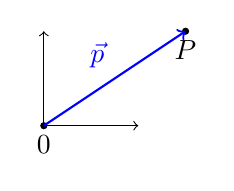
\begin{tikzpicture}[scale=0.6]
          \draw[<->](2,0,0)--(0,0,0)--(0,2,0);
          \draw[fill] (0,0) circle [radius=1.8pt] node[below]{$0$};
          \draw[fill] (3,2) circle [radius=1.8pt] node[below]{$P$};
          \draw[thick, blue, ->](0,0) -- node[above left]{$\vec{p}$} (3,2);
        \end{tikzpicture}
      \end{center}
      If the point $P$ has coordinates $(p_1,\ldots,p_n)$, then the
      components of the position vector are
      \begin{equation*}
        \vec{p} =
        \startmat{c}
          p_1    \\
          \vdots \\
          p_n
        \stopmat.
      \end{equation*}
      Thus, the coordinates of a point are the same as the components of
      its position vector. 
      
      \begin{remark}
      
      For this reason, we will often interchangeably visualize vectors as points in space, or visualize them as arrows. For the purposes of this course, the choice of one over the other is often cosmetic, or a matter of emphasis. If there are too many vectors to nicely visualize at once as arrows, we'll often use points instead.

    \end{remark}
    \end{definition}

    The value in each coordinate tells you how far along its axis you should move.


    %Include a jpg image of a 3-dimensional vector [80, 3, 25] in a 3-dimensional space
    \begin{center}
      %make the width 3/4 of the textwidth
    \includegraphics[width=.75\textwidth]{80-3-25_vector.png}
    \end{center}

    You locate our vector $\vec{a}=[80, 3, 25]$ by first moving 80 units along the $x$-axis, then moving 3 units in the direction of the $y$-axis along the $x-y$ plane, and finally moving 25 units in the direction of the $z$-axis in $x-y-z$ space, as seen in Figure BLAH. (Note: the axes are not uniformly scaled in this figure).


\end{description} 
\end{remark}

\begin{exploration}

  Let's say one apple weighs 160 grams (aka 1.6 \emph{decagrams}), has a stem length of 3 cm, and has a circumference of 25 cm (aka 2.5 \emph{meters}). Which of the vectors depicted below could represent the apple? (Select all that apply)

  \choice[correct]{

  \begin{center}
    %make the width 3/4 of the textwidth
    \includegraphics[width=.75\textwidth]{apple_vector_1.png}
  \end{center}
  }
  
\choice[correct]{
    
    \begin{center}
      %make the width 3/4 of the textwidth
    \includegraphics[width=.75\textwidth]{apple_vector_2.png}
    \end{center}
}

\choice[correct]{

  \begin{center}
    %make the width 3/4 of the textwidth
    \includegraphics[width=.75\textwidth]{apple_vector_3.png}
  \end{center}

}

\begin{solution}

  All of above could be valid geometric representations of the apple. The main utility is that once each coordinate is assinged a feature (like weight, color, volume, etc.), we want all apples (or fruit for that matter) to have the same ordered features. This way we can compare apples to apples, so to speak, or more generally fruits to fruits.

\end{solution}

\end{exploration}

\begin{exploration}

Finally, let's see one (among countless) application of vector representations.

  A common way to apply vector representations is through classification. This involves making vectors out of the features of objects that you wish to classify (fruits, flowers, houses), and then determining a way to classify multiple objects based on the geometry of the vector representations.


\begin{example}

    Suppose we want to use feature information to compare apples and pears. A data scientist might hope that there's an easy way to geometrically separate all of the apple vectors from pear vectors in a given data set. They'd then use that geometry to predict whether a new fruit is an apple or a pear based on its measurement. 

    It's never as simple geometrically as the GeoGebra environment below, but the idea is the same. We'll do an advanced version of this later in the course when we talk about voting patterns and facial recognition.

    

    \begin{center}
        \pdfOnly{\includegraphics[width=.75\textwidth]{apple-pear.png}\\
        $$\vec{F}\text{ is within the Apple cluster, and is thus an apple rather than a pear.}$$}
        \geogebra{qnghrmdg}{800}{600} %%https://www.geogebra.org/m/qnghrmdg
    \end{center}

    In this very idealistic example, the apple vectors (visualized as red points in 3-D space) cluster together nicely, as do the (blue) pear vectors. You can think of this clustering loosely as the pear vectors generally being closer (distance-wise) to other pears than to apples (we'll talk about this below, and in the homework and discussion).
    
    You can also think of their ``clustering" in terms of a separation in space. If you put a 2-D plane between the apple and pear clusters, the plane cleanly separates the two clusters. We'll revisit this process later in the course as well more explicitly. 
    
    The main point is that the ideas of ``clustering" and ``separation" enable someone to build a program that sorts apples and pears taken from farms en masse based on the feature measurements of the fruit. This exemplifies a powerful use of structure in vectors, that of prediction. As seen in the applet, we don't only care about the apple and pear vectors that we know about, we also care that if we get a new fruit, we can accurately predict whether it's an apple or pear based on the location of its vector representation in 3D space. If it's close to one cluster, or on one side of the plane, and not absurdely far from either cluster (imagine that a banana accidentally got mixed in with the apples and pears), we can predict its type with some confidence.

    
\end{example}
\end{exploration}

\subsection{Vectors in the Physical World}

If you're coming from STEM, you've probably more accustomed to thinking about vectors in relation to physical quantities like speed, acceleration, force, and electric fields. Whereas in other settings (such as the apple example above), the vector representations can be somewhat abstract, or arbitrary, and the structure of the geometry is key, in the physical world the geometry of vectors themselves are much more closely linked to a physical interpretation.

\subsubsection{A Physical Example: Velocity}

Velocity, acceleration, and forces naturally lend themselves to vector representation, and point us towards other properties of vectors that we care to measure, namely those of \textit{magnitude} and \textit{direction}. This example will emphasize the utility of \textit{addition} and \textit{scaling} as fundamental to vectors.

\begin{example}
    
  Suppose an airplane is flying from Daytona Beach to a location roughly northeast of Daytona Beach at a speed of $300$ knots. If we were in a scalar context, $300$ would be the only necessary speed information, as we could distinguish $300$ from $-300$ as being "forward" or "backward" motion, and the value $300$ to give the speed. In the spatial world, however, objects move in directions, and so we need to know the direction of the airplane's velocity as well.

  In the following GeoGebra application, scaled down so that $300$ knots has a value of $3$, the airplane's destination is located at around $(11.14,4.46)$, and the airplane's starting location is at $(0,0)$. 

  \begin{center}
    \geogebra{qytw4pbt}{801}{575}
  \end{center}

  The vector $\vec{D}=[11.14,4.46]$ gives the airplane a direction, but we also need to factor in the ariplane's speed. We want the geometric length of the vector to be the plane's speed ($300$ knots), so we want the plane's velocity vector to be an arrow in the direction of $\vec{D}$, but only a length $3$. The vector length is called its \textit{magnitude}, and for our purposes its magnitude directly correlates to speed. As such, we need a way to geometrically determine the lengths of vectors, for which we'll use the Pythagorean theorem.

  \begin{remark}

    Distance and length are two sides of the same coin for standard Euclidean space, and the Pythagorean theorem key.

    Consider two points $P=(p_1,p_2)$ and
    $Q=(q_1,q_2)$ in the plane, as in the following picture.
    \begin{equation*}
      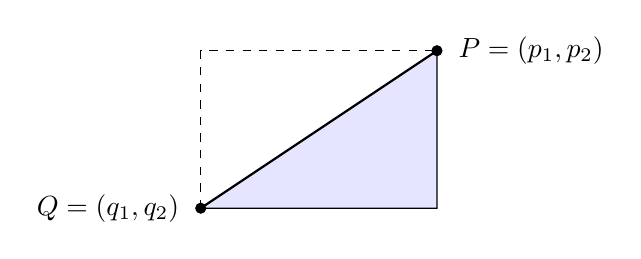
\begin{tikzpicture}[scale=1]
        \draw[dashed] (0,0) -- (0,2) -- (3,2);
        \draw[fill=blue!10] (0,0) -- (3,0) -- (3,2) -- cycle;
        \draw[thick] (0,0) -- (3,2);
        \draw[fill](0,0) circle [radius=1.8pt] node[left=1ex]{$Q=(q_1,q_2)$};
        \draw[fill](3,2) circle [radius=1.8pt] node[right=1ex]{$P=(p_1,p_2)$};
      \end{tikzpicture}
    \end{equation*}
    The distance between $P$ and $Q$ is shown in the picture as a solid
    line, which is the hypotenuse of a right triangle.  The lengths of the
    two other sides of this triangle are $(p_1-q_1)$ and
    $(p_2-q_2)$. Therefore, the Pythagorean Theorem implies the
    length of the hypotenuse (and thus the distance between $P$ and $Q$)
    equals
    \begin{equation*}
      d(P,Q)
      =\sqrt{(p_1-q_1)^2+(p_2-q_2)^2}.
    \end{equation*}

    Similarly in 3 dimensions, points $P=(p_1,p_2,p_3)$ and
    $Q = (q_1,q_2,q_3)$ have a distance of $d(P,Q)=\sqrt{(p_1-q_1)^2+(p_2-q_2)^2+(p_3-q_3)^2}$.

    \begin{equation*}
      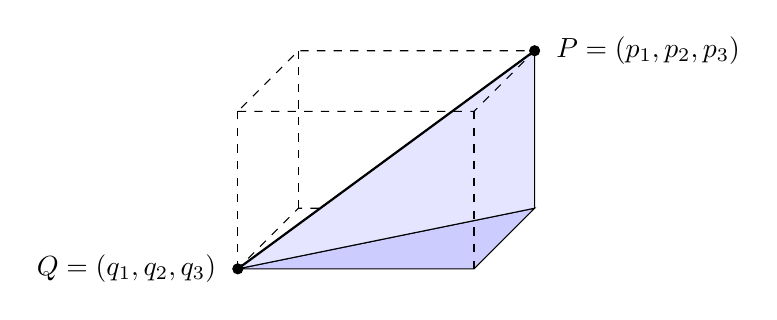
\begin{tikzpicture}[scale=1]
        \draw[dashed] (3,0,-2) -- (0,0,-2) -- (0,0,0);
        \draw[dashed] (0,0,0) -- (0,2,0);
        \draw[dashed] (0,0,-2) -- (0,2,-2);
        \draw[fill=blue!20] (0,0,0) -- (3,0,0) -- (3,0,-2) -- cycle;
        \draw[fill=blue!10] (0,0,0) -- (3,0,-2) -- (3,2,-2) -- cycle;
        \draw[dashed] (0,2,0) -- (3,2,0) -- (3,2,-2) -- (0,2,-2) -- cycle;
        \draw[dashed] (3,0,0) -- (3,2,0);
        \draw[thick] (0,0,0) -- (3,2,-2);
        \draw[fill](0,0,0) circle [radius=1.8pt] node[left=1ex]{$Q=(q_1,q_2,q_3)$};
        \draw[fill](3,2,-2) circle [radius=1.8pt] node[right=1ex]{$P=(p_1,p_2,p_3)$};
        %\draw[fill](3,0,-2) circle [radius=1.8pt] node[right=1ex]{$R=(p_1,p_2,q_3)$};
        %\draw[fill](3,0,0) circle [radius=1.8pt] node[right=1ex]{$S=(p_1,q_2,q_3)$};
      \end{tikzpicture}
    \end{equation*}

  
\begin{definition}\name{Distance between points}
  
      Let $P=(p_1,\ldots,p_n)$ and $Q=(q_1,\ldots,q_n)$ be two points in
      $\R^n$. Then the \textbf{distance}%
      \index{distance!point to point} between these points is defined as
      \begin{equation*}
        d(P, Q) = \sqrt{(p_1-q_1)^2 + \ldots + (p_n-q_n)^2}.
      \end{equation*}
      This formula is also called the \textbf{distance formula}%
      \index{distance formula}. We may also write $\left\|PQ\right\|$ for the
      distance between $P$ and $Q$.
    \end{definition}

A vector's \textit{magnitude}, then, can be thought of as its distance from $\vec{0}$. 

\begin{definition}\name{Length of a vector}
  Let
  \begin{equation*}
    \vec{u} = \startmat{c} u_1 \\ \vdots \\ u_n \stopmat
  \end{equation*}
  be a vector in $\R^n$. Then the \textbf{length}%
  \index{vector!length}%
  \index{length of a vector} of $\vec{u}$, written $\left\| \vec{u} \right\|$,
  is given by
  \begin{equation*}
    \left\| \vec{u} \right\| = \sqrt{u_1^2 + \ldots + u_n^2}.
  \end{equation*}
  The length of a vector is also sometimes called its
  \textbf{magnitude}%
  \index{magnitude!of a vector}%
  \index{vector!magnitude} or its
  \textbf{norm}%
  \index{norm!in Rn@in $\R^n$}%
  \index{vector!norm}.
\end{definition}

  \end{remark}

  So, to describe our plane's velocity vector, it needs to be in the same direction as the vector $\vec{D}=[11.14,4.46]$, but with a length of $3$. Using the definition above, the length of the destination vector is $\left\|\vec{D}\right\|=\sqrt{11.14^2+4.46^2}\approx 12$. To get a vector of length $3$, to re-size its coordinates to match the right scale, so we divide each coordinate by $\left\|\vec{D}\right\|$ and multiply by $3$, yielding the vector $$\vec{v}=\left[11.14\cdot \frac{3}{12},4.46\cdot \frac{3}{12}\right]\approx \left[\frac{11.14}{4},\frac{4.46}{4}\right] = [2.79,1.12].$$

  Note that to re-size $\vec{v}$ so that it has a length of $3$, we also determined the amount by which we scaled the destination vector $\vec{D}$ to get $\vec{v}$. Knowing that each coordinate of $\vec{v}$ is $\frac{1}{4}$ of the corresponding coordinate of $\vec{D}$ (say, in ``knots-per-hour''), the plane will reach the destination in $\answer{4}$ hours.

  Hence, the geometric vector in the applet represents the plane's speed and direction. This is an example of \emph{scalar multiplication} of a vector, where we multiply each coordinate of the vector by a scalar.

  \begin{remark}

    This leads to a definition.

    \begin{definition}\name{Scalar Multiplication of a Vector}

      Let $\vec{v} = \startmat{c} v_1 \\ \vdots \\ v_n \stopmat$ be a vector in $\R^n$ and let $c$ be a scalar. The \textbf{scalar multiple} of $\vec{v}$ by $c$ is the vector
      \begin{equation*}
        c\vec{v} = \startmat{c} cv_1 \\ \vdots \\ cv_n \stopmat.
      \end{equation*}

    \end{definition}

    In other words, we multiply a vector by a scalar by multiplying each of its coordinates by the scalar. The vector represents velocity because the scale is with respect to time, so each coordinate gives how far in the coordinate directions the plane will travel in one hour.

  \end{remark}

\end{example}

\begin{example}
  
  Suppose that for the entire trip, the wind is blowing exactly in the northwestern direction at a speed of $100*\sqrt(2)$ knots ($\sqrt{2}$ in the applet). The wind (uniformly applied throughout the trip) is imposing another velocity on the plane. To determine the plane's new trajectory, we need the notion of \textit{vector addition}.

  The plane's velocity vector is given in the GeoGebra environment below. You can always see its intended trajectory (and original velocity vector) in purple. Hit the ``Animate'' button to see the plane's path.

  A northwestern wind moves equally to the right as it does upward, so with a speed of $\sqrt{2}$ the wind vector is $\vec{w}=[\answer{1},\answer{1}]$.

  \begin{solution}

    You can use $[a,a]$ for the direction vector moving equally westward and northward, and then keeping the pythagorean theorem in mind, $\sqrt{2}=\sqrt{1^2+1^2}$, you can determine the wind vector $\vec{w}=[1,1]$.

  \end{solution}

  Select the "Allow Wind" checkbox and enter $\vec{w}$ as the wind vector, and then hit "Set Wind". This will visualize a new trajectory for the plane. The black vector is the plane's new velocity vector, the purple vector is the plane's original velocity vector, and the blue vector is the wind vector. Note that to get the black vector, you first move along the purple vector, and then move along the blue vector starting at the head of the purple vector.

  Since the plane maintains the velocity vectors throughout the flight, you can see the plane's final destination by hitting the "Animate" button, noting that the velocity is constantly affecting the distance traveled.
  \begin{center}
    \geogebra{qytw4pbt}{801}{575}
  \end{center}

  \begin{remark}

This is how we geometrically interpret \emph{vector addition}. If $\vec{v}$ is the plane's velocity vector, and $\vec{w}$ is the wind vector, then the plane's new velocity vector is $\vec{v}+\vec{w}$. 

Numerically, you find this by adding the coordinates of the vectors. So, if $\vec{v}=[2.79,1.12]$ and $\vec{w}=[1,1]$, then 

$$\vec{v}+\vec{w}=[2.79+1,1.12+1]=[\answer{3.79},\answer{2.12}].$$

\begin{definition}\name{Addition of vectors in $\R^n$}
  For vectors $\vec{u}=\startmat{c}
    u_1 \\
    \vdots \\
    u_n
  \stopmat,\; \vec{v}= \startmat{c}
    v_1 \\
    \vdots \\
    v_n
  \stopmat$ in $\R^n$, the sum%
  \index{vector!addition}%
  \index{addition!of vectors} $\vec{u}+\vec{v}$ in $\R^n$ is defined
  by
  \begin{equation*}
    \vec{u}+\vec{v} = \startmat{c}
      u_1 \\
      \vdots \\
      u_n
    \stopmat +  \startmat{c}
      v_1 \\
      \vdots \\
      v_n
    \stopmat
    = \startmat{c}
      u_1+v_1 \\
      \vdots \\
      u_n+v_n
    \stopmat.
  \end{equation*}
\end{definition}

The geometry and the numerical interpretations together make sense, since you can imagine getting to the tip of the sum vector by 


\begin{tikzpicture}

  % Draw x and y axes
  \draw[->] (-1,0) -- (6,0); %node[right] {$x$};
  \draw[->] (0,-1) -- (0,6); %node[above] {$y$};
  
  % Define the origin
  \coordinate (O) at (0,0);
  
  % Define vectors u and v
  \coordinate (U) at (3,1);   % Vector u components (3, 2)
  \coordinate (V) at (1,3);   % Vector v components (2, 1)
  
  % Calculate u + v
  \coordinate (UV) at ($(U)+(V)$);
  
  % Draw vector u
  \draw[->, thick, red] (O) -- (U) node[midway, above] {$\vec{u}$};
  
  % Draw vector v starting from tip of u
  \draw[->, thick, red] (U) -- (UV) node[midway, right] {$\vec{v}$};
  
  % Draw resultant vector u + v
  \draw[->, thick, blue] (O) -- (UV) node[midway, above left] {$\vec{u} + \vec{v}$};
  
  % Draw dashed lines to form right triangles for u
  \draw[dashed] (U) -- (U |- O) -- (O);
  
  % Draw dashed lines to form right triangles for v
  \draw[dashed] (UV) -- (UV |- U) -- (U);
  
  % Draw dashed lines to form right triangles for u + v
  %\draw[dashed] (UV) -- (UV |- O) -- (O);
  
  % Mark right angles
  % For vector u
  \draw ($(U) + (-0.2,0)$) -- ++(0,-0.2) -- ++(0.2,0);
  % For vector v
  \draw ($(UV) + (-0.2,0)$) -- ++(0,-0.2) -- ++(0.2,0);
  
\end{tikzpicture}

You can move horizontally below (or above) the first coordinate of $u+v$ by moving $u_1$ then $v_1$ (hence, $u_1+v_1$), and similarly for the second coordinate. This is the geometric interpretation of vector addition.

  \end{remark}

\end{example}

\begin{example}

  By how much do you need to correct the plane to reach its destination in a straight shot? There are two immediately avaialable options, with one making more practical sense than the other. 

  First, you can direct the plane against the wind, so that the wind velocity is canceled out and the plane can return to its original course. This adds the negative of $\vec{w}$ to $\vec{v}$, so that the plane's new velocity vector is $\vec{v}+\vec{w}-\vec{w}=\vec{v}$.

  Try this in the applet, by selecting the "Allow Correction" check box and entering $-\vec{w}=[-1,-1]$. Setting the wind and correction then shows the plan on its original course, with the velocity vectors first moving along the initial velocity, then along the wind, then back down reversing the velocity. 

  \begin{center}
    \geogebra{qytw4pbt}{801}{575}
  \end{center}

  You could take a more efficient route, however, by noting that the wind does push the plane further north and west than it would have gone otherwise, so there is some added speed in a direction similar to the intended direction. If you set the correction vector correctly, you re-orient the plane along its intended path but also with less travel time than the original path.

  First, do so in the applet, then solve for the correction vector $\vec{c}$ algebraically below.

  
  We want $\vec{v}+\vec{w}+\vec{c}$ to be in the same direction as $\vec{v}$, but with a magnitude greater than $3$. Assuming that we want to minimally increase the plane's engine use, let's just give the correction vector a vertical component (really we would want to go at a right angle to the wind vector, but we'll cover that later). 

  So, we want $\vec{v}+\vec{w}+\vec{c}=[2.79+1,1.12+1+c_2]=[3.79,2.12+c_2]$ to be in the same direction as $\vec{v}=[2.79,1.12]$. This is hard to do unless we have a common scale, so we need to think \emph{just} about direction for a moment, rather than direction and length together. This is the notion of \textit{unit vectors} (or \textit{direction vectors}).

  \begin{definition}\name{Unit Vectors}

    A \textbf{unit vector}%
    \index{unit vector}%
    \index{vector!unit} is a vector of length $1$. 

    In $\R^n$, the standard coordinate vectors are examples of unit vectors. In $\R^3$, the coordiante vectors are $\vec{i}=[1,0,0]$, $\vec{j}=[0,1,0]$, and $\vec{k}=[0,0,1]$.
  \end{definition}

  Since we want $\vec{v}+\vec{w}+\vec{c}$ and $\vec{v}$ to be in the same direction, we can solve for the coordiantes of $\vec{v}+\vec{w}+\vec{c}$ in the following way: 

\begin{enumerate}

\item Find the unit vector $\vec{u}$ in the direction of $\vec{v}$. Since $\vec{v}$ is fixed, we can find $\vec{u}$ by dividing $\vec{v}$ by its length.
\item Since $\vec{v}+\vec{w}+\vec{c}$ is in the same direction as $\vec{v}$, which is in the same direction as $\vec{u}$, all three vectors are scalar multiples of each other. Geometrically, each vector is a stretched or compressed version of the others. So we can solve for the scalar $s$ such that $\vec{v}+\vec{w}+\vec{c}=s\vec{u}$.
\item The vector equation $\vec{v}+\vec{w}+\vec{c}=s\vec{u}$ gives us two scalar linear equations, which we can solve for the two unknowns $s$ and $c_2$.

\begin{hint}

  We'll develop more sophisticated ways of doing this in Chapter 3, but for now you solve a system of two scalar linear equations by first isolating one variable, substituting it into the other equation, and solving for the other variable to then substitute back.

  For instance, the steps to solving 

  $$\begin{array}{rcl}
    2x+y&=&3\\
    x-2y&=&-1
  \end{array}$$

  would be to first isolate $x$ in the second equation, so that $x=2y+1$, then substitute this into the first equation to get $2(2y+1)+y=3$, which simplifies to $5y+2=3$, so $y=1/5$. Substituting this back into $x=2y+1$ gives $x=7/5$.

\end{hint}

\end{enumerate}

  \begin{solution}

  $\left\|\vec{v}\right\|=\sqrt{2.79^2+1.12^2}\approx 3$, so $\vec{u}=\left[\frac{2.79}{3},\frac{1.12}{3}\right]\approx [0.93,0.37]$. 

  The vector equation $\vec{v}+\vec{w}+\vec{c}=s\vec{u}$ can be stated in components as $s[.93,.37]=[3.79,2.12+c_2]$. This gives us two equations

  \begin{align*}
    .93s&=3.79\\
    .37s&=2.12+c_2
  \end{align*}

  The first equation gives $s\approx 4.08$, and substituting this into the second equation gives $c_2\approx .37s-2.12=.37(4.08)-2.12\approx -.61$. So, the correction vector is $\vec{c}=[0,-.61]$.

  \end{solution}

  When all is said and done, the plane's new velocity vector is $\vec{v}+\vec{w}+\vec{c}=[2.79, 1.12]+[1,1]+[0,\answer{-.61}]\approx [3.79,\answer{1.51}]$. With this velocity, the plane will travel along the same path but get to the destination in less time.
  
\end{example}

\begin{exploration}

  Wrapping up this initial discussion of vectors, let's consider other quantities for which it does or does not make sense to \emph{add} and \emph{scale}.

  \begin{example}\name{When adding doesn't make sense}

\begin{description}
\item[Personal Identification Numbers] Summing things like social
  security numbers, phone numbers, or zip codes doesn't provide
  meaningful information.
\item[Temperatures] While you can mathematically add temperatures
  together, doing so usually doesn't provide useful information.
\item[Time] Adding specific points in time, like dates or hours of the
  day, usually doesn't yield meaningful results.
\item[Geographic Coordinates] Adding the latitude and longitude of two
  locations doesn't give you a location that has any real-world
  significance.
\end{description}
\end{example}

For some of the categories above, the \textit{average} can be
meaningful; or perhaps if each quantity is thought of as
`displacement' or `duration,' summing might be meaningful. However,
without additional (pun intended!) stipulations, summing the types of
quantities above is not meaningful.

\begin{example}

On the other hand, there are lots of
times that it makes sense to add data:


\begin{description}
\item[Population Counts] Adding the populations of different regions,
  cities, or countries to find the total population of a larger
  area. Answers to questions like these help us understand our
  society and are important to many people.
\item[Financial Transactions] Summing daily sales to find total
  monthly sales, or adding up all expenses to find total costs. These
  are real numbers that represent actual amounts of money, and their
  total gives meaningful information about financial status or
  performance.
\item[Time Spent on Tasks] Adding the duration of time spent on
  various activities on day gives a total time spent. We all have busy
  lives, and time is a very precious commodity. Hence, it is good to
  understand how we spend our time.
\item[Navigation] Aircraft navigate by knowing the direction and speed
  that they are traveling. When interpreted correctly, we add the
  speed and direction of many of many different ``course changes'' to
  find the ultimate position of the aircraft.
\end{description}

\end{example}

Often when it make sense to \textit{add} quantities, it make sense to
\textit{scale} them as well. For example with population, you could
ask for the population of a city with $3$ times the population, or
half the population. Similar \textit{scaling} examples exist for all
the examples above where it make sense to add data.

\end{exploration}

In the next section, we introduce the idea of a \emph{matrix}, which for now we will roughly discuss as a specific way to organize multiple data vectors together. This will be the first step in understanding how to manipulate and analyze data in a more sophisticated way than we have so far.





\end{document}